\documentclass[10pt,portrait, twocolumn]{article}
\usepackage{multicol}
\usepackage{calc}
\usepackage[portrait]{geometry}
\usepackage{amsmath,amsthm,amsfonts,amssymb}
\usepackage{times}
\usepackage{color,graphicx,overpic}
\graphicspath{ {images/} }
\usepackage{hyperref}
\usepackage{pgfplots}
\usepackage{esint}
\usepackage{bm}
\usepackage{tikz}
\usepackage{relsize}
\usepackage{datetime}
\usepackage[utf8] {inputenc}
\usepackage[spanish, activeacute] {babel}
\usepackage{IEEEtrantools}
\usepackage{framed}

\usepackage{pdflscape}

\usepackage{draftwatermark}
\SetWatermarkText{Javier de Martín}
\SetWatermarkScale{0.8}

% This sets page margins to .5 inch if using letter paper, and to 1cm
% if using A4 paper. (This probably isn't strictly necessary.)
% If using another size paper, use default 1cm margins.
\geometry{top=.5cm,left=.5cm,right=.5cm,bottom=.5cm}
    
\pgfplotsset{
    dirac/.style={
        mark=triangle*,
        mark options={scale=2},
        ycomb,
        scatter,
        visualization depends on={y/abs(y)-1 \as \sign},
        scatter/@pre marker code/.code={\scope[rotate=90*\sign,yshift=-2pt]}
    }
}

% Turn off header and footer
\pagestyle{empty}

% Redefine section commands to use less space
\makeatletter
\renewcommand{\section}{\@startsection{section}{1}{0mm}%
                                {-1ex plus -.5ex minus -.2ex}%
                                {0.5ex plus .2ex}%x
                                {\normalfont\large\bfseries}}
\renewcommand{\subsection}{\@startsection{subsection}{2}{0mm}%
                                {-1explus -.5ex minus -.2ex}%
                                {0.5ex plus .2ex}%
                                {\normalfont\normalsize\bfseries}}
\renewcommand{\subsubsection}{\@startsection{subsubsection}{3}{0mm}%
                                {-1ex plus -.5ex minus -.2ex}%
                                {1ex plus .2ex}%
                                {\normalfont\small\bfseries}}
\makeatother

\newcommand{\Lagr}{\mathcal{L}}

% Define BibTeX command
\def\BibTeX{{\rm B\kern-.05em{\sc i\kern-.025em b}\kern-.08em
    T\kern-.1667em\lower.7ex\hbox{E}\kern-.125emX}}

% Don't print section numbers
\setcounter{secnumdepth}{0}


\setlength{\parindent}{0pt}
\setlength{\parskip}{0pt plus 0.5ex}

%My Environments
\newtheorem{example}[section]{Example}
% ---------------------------------------------------------------

\begin{document}


\begin{framed}
	\begin{center}
    	\Large{\underline{Sistemas de Radiocomunicación}} \\
	\large{Primera Parte} \\
    	\scriptsize{3º Ingeniería de Telecomunicaciones | UPV/EHU}\\
     	%Actualizado por última vez el \today \\
     	"\textsl{Under-promise and over-deliver}." \\
     	%\hspace{5 pt} \\
     	\small{\textbf{Javier de Martín -- 2016}}
	\end{center}
\end{framed}

%%%%%%%%%%%%%%%%%%%%%%%%%%%%%%%%%%%%%%%%%%%%%%%%%%%%%%%%%%%%%%%%%
% Tema 4

\section{\underline{1. Ingeniería del Espectro Radioeléctrico}}

\textbf{Radiocomunicación}: Telecomunicación basada en ondas de radio.\\
\textbf{Telecomunicación}: Cualquier transmisión o recepción de información por aire, radio, cable o cualquier otro sistema de electromagnetismo.\\
\textbf{Radio}: Término general aplicado al uso de ondas de radio.\\
\textbf{Ondas de Radio}: Ondas EM con frecuencias arbitrariamente menores a 3000 GHz (excepto la luz), que se propaga en el espacio sin necesidad de guías artificiales.

El espectro de radio varía desde los 3kHz hasta los 300GHz

Bandas de frecuencia según EBU (European Broadcasting Union)

	\begin{center}
\begin{tabular}{|l|l|}
\hline
Banda I   & 41-68MHz    \\ \hline
Banda II  & 87,5-108MHz \\ \hline
Banda III & 162-230MHz  \\ \hline
Banda IV  & 470-582MHz  \\ \hline
Banda V   & 582-960MHz  \\ \hline
Banda VI  & 12 GHz      \\ \hline
\end{tabular}
	\end{center}
	
Bandas según ITU, nomenclatura de Radar

	\begin{center}
	\begin{tabular}{|l|l|}
\hline
L  & 1-2 GHz    \\ \hline
S  & 2-4 GHz    \\ \hline
C  & 4-8 GHz    \\ \hline
X  & 8-12 GHz   \\ \hline
Ku & 12-18 GHz  \\ \hline
K  & 18-27 GHz  \\ \hline
Ks & 27-40 GHz  \\ \hline
mm & 40-300 GHz \\ \hline
\end{tabular}
	\end{center}
	
El espectro de radiocomunicación es un recurso natural limitado pero reutilizable. La limitación es debida a las características de propagación de las ondas de radio, disponibilidad de la tecnología y equipamiento para diferentes aplicaciones y disponibilidad de bandas de frecuencias adecuadas para aplicaciones específicas. La demanda del espectro siempre ha sido mayor que su disponibilidad.\\

Sólo hay un único espectro de radio, es únicamente expandible hasta las ondas de longitud de onda milimétrica o empleando métodos de codificación. Las ondas de radio no respetan las fronteras internacionales, edificios u otros.

\subsection{Gestión del Espectro}

La \textbf{ITU} (International Telecommunication Union) atribuye el espectro global y órbitas de satélite, desarrollar estándares técnicos que aseguren la interconexión de redes y tecnologías y forzar la mejora del acceso a ICTs en comunidades subdesarrolladas.\\

Las \textbf{WRC} (World Radiocommunication Conferences) de la ITU se celebran cada tres años en Ginebra, revisan las regulaciones de radio, el uso del espectro y cualquier otro aspecto.\\

La \textbf{ETSI} (European Telecommunication Standards Institute) crea estándares para tecnologías de radio. Fundada inicialmente para cubrir las necesidades europeas ha crecido para ser respetada como un estándar mundial.

\begin{center}
\begin{tabular}{l|c|c|}
\cline{2-3}
                                            & \textbf{English} & \textbf{Spanish} \\ \hline
\multicolumn{1}{|l|}{\textbf{Servicios}}    & Allocation       & Atribución       \\ \hline
\multicolumn{1}{|l|}{\textbf{Áreas/Paises}} & Allotment        & Adjudicación     \\ \hline
\multicolumn{1}{|l|}{\textbf{Estaciones}}   & Assignment       & Asignación       \\ \hline
\end{tabular}
\end{center}

\begin{itemize}
	\item \textbf{Allocation} (of a frequency band): Entrada en la tabla de atribución de frecuencias de una banda de frecuencia dada para el propósito por uno o más servicios de radiocomunicación terrestres o espaciales. Este término también se aplica a la banda de frecuencias afectada.
	\item \textbf{Allotment} (of a radio frequency or radio frequency channel): Entrada de un canal de frecuencias en un plan acordado, es adoptado por una conferencia competente, para usarlo en uno o más administraciones para radiocomunicación terrestre o espacial un uno o más países o áreas geográficas bajo unas condiciones especificadas.
	\item \textbf{Assignment} (of a radio frequency or a radio frequency channel): Autorización proporcionada por una administración para que una estación de radio pueda utilizar una frecuencia o un canal de radiofrecuencia bajo unas condiciones especificadas.
\end{itemize}

\begin{figure}[h]
	\centering
     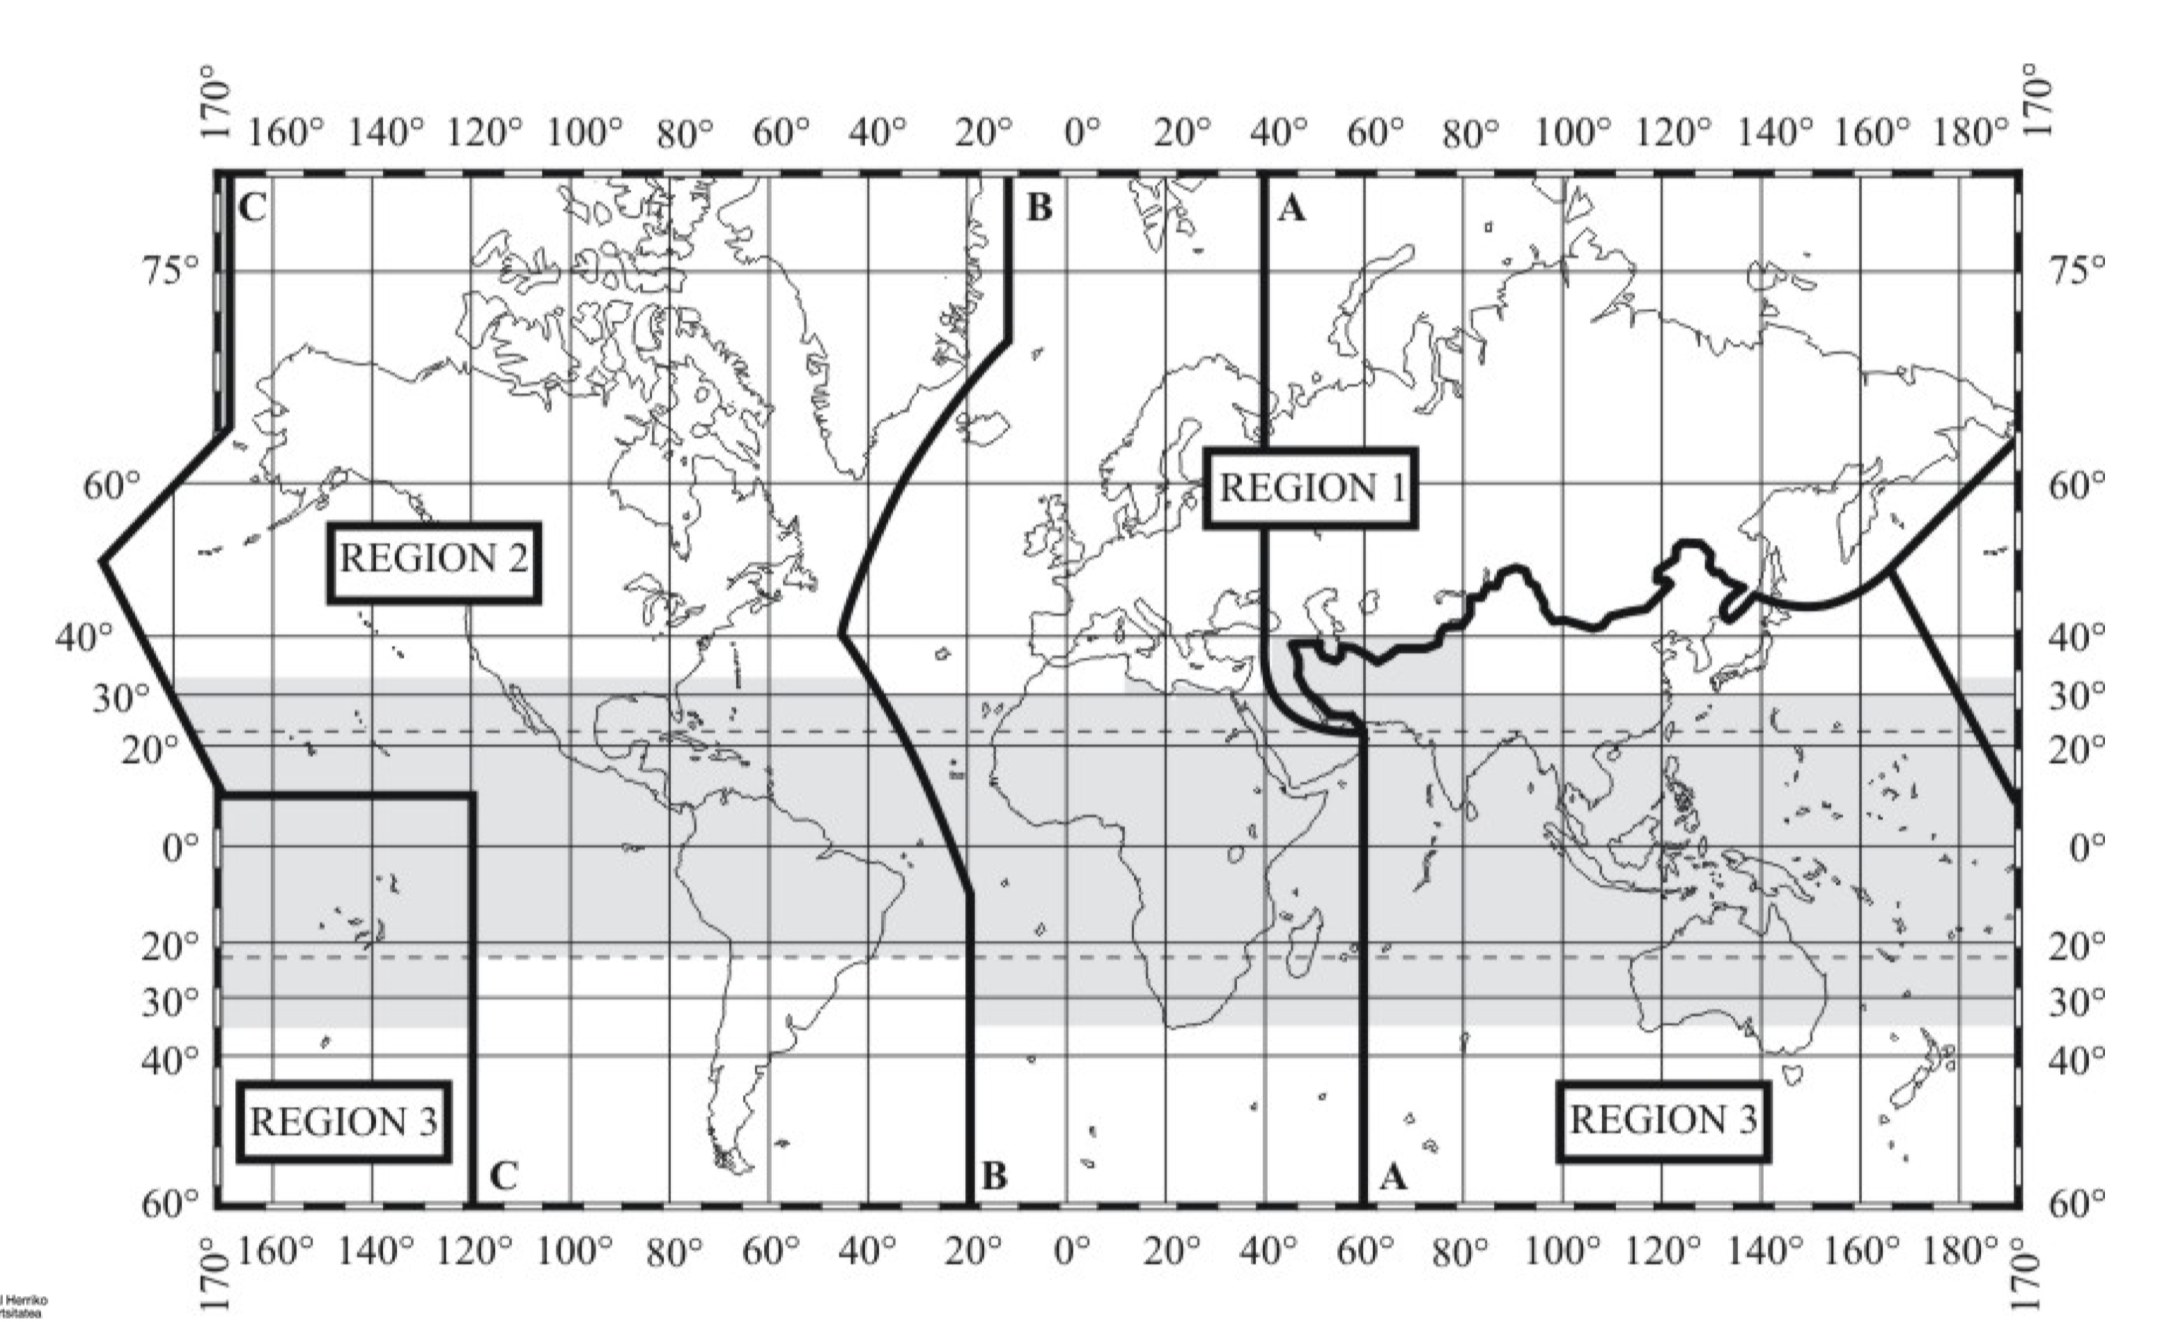
\includegraphics[width=0.5\textwidth]{Regiones}
      \caption{Regiones de frecuencias}
      \label{fig:Regiones de frecuencias}
  \end{figure}

Hay varios \textbf{tipos} de atribuciones de frecuencias:

	\begin{itemize}
		\item \textbf{Exclusiva}: Atribución para un servicio de radio.
		\item \textbf{Compartido}: Atribución para varios servicios de radio.
	\end{itemize}
	
\textbf{Categorías} de servicios:

	\begin{itemize}
		\item \textbf{Primarios}: Prioridad en la elección de las frecuencias, escrito en mayúsculas.
		\item \textbf{Secundario}: No pueden producir interferencias a estaciones primarias. No pueden reclamar protección por interferencia a estaciones de servicios primarios. Pueden reclamar protección contra interferencias de estaciones del mismo servicio u otros servicios secundarios.
	\end{itemize}
	
La \textbf{gestión del espectro} refleja muchas actividades: Planificación del uso del espectro, atribución y asignación de licencias del espectro, interacción con organizadores regionales e internacionales... Históricamente, los reguladores han asignado las frecuencias emitiendo licencias a usuarios específicos para usos específicos $\rightarrow$ Método Administrativo. Hay formas más flexibles de licencia, las bandas se pusieron a disposición de varios usos en vez de sólo para uno y se introdujeron subastas para asignar los espectros a los usuarios.\\

El \textbf{modelo administrativo} es el utilizado por la mayoría de reguladores en el mundo. Los reguladores son las autoridades centrales para la asignación del espectro y decisiones de uso. Las decisiones de asignación son a menudo estáticas en dimensiones temporales y espaciales, es decir, son válidas para períodos de tiempo muy largos y para grandes regiones geográficas por lo que no resulta muy eficiente.\\

El \textbf{modelo de mercado} dice que los recursos del espectro de radiocomunicación debería ser tratado como propiedad privada. La asignación debe de er implementada por las fuerzas de mercado. Los propietarios del espectro deberían ser capaces de comerciar esas partes en mercados secundarios. Los propietarios de espectro podrán utilizar su banda de la manera que quieran a través de cualquier tecnología.\\

La \textbf{teoría del espectro libre} proporciona acceso libre a cualquier espectro para cualquier uso, está necesitada de regulaciones para poner orden.\\

A vistas de \textbf{futuro} se preveé una mayor demanda del espectro disponible, planes centrados en incrementar la compartición del espectro entre servicios, planes centrados en la liberación del espectro no utilizado o no utilizado eficientemente.\\

Las \textbf{licencias} se asignan a estaciones de radio para usuarios específicos con usos específicos y asignadas en subastas. El espectro \textbf{sin licencia} tiene frecuencias para aplicaciones ISM y SDR, limitando la potencia emitida, cualquiera puede transmitir sin una licencia mientras cumpla con las reglas para limitar/evitar interferencias, las principales bandas sin licencias fueron aquellas diseñadas como industriales, científicas y médicas (ISM). En los últimos 15 años ha crecido la demanda en el uso del espectro sin licencia.

\hrulefill
	
	
	
%\vfill




%\end{multicols}

\end{document}